\documentclass[11pt]{article}
\usepackage[margin=1in]{geometry}
\usepackage{amsmath,amsfonts,graphicx,hyperref}
\usepackage{titlesec}
\titleformat{\section}{\large\bfseries}{}{0em}{}
\titleformat{\subsection}{\normalsize\bfseries}{}{0em}{}

\title{QOFAS: Passive Superposition Detection and Field Readout for Quantum Information Systems}
\author{Jonathon Poe \\ \texttt{noblesite@gmail.com}}
\date{}

\begin{document}
\maketitle

\section*{Abstract}
Quantum Optical Field Amplification Shell (QOFAS) is a novel framework for detecting quantum states, entangled systems, and electromagnetic field interactions through passive optical distortion analysis. Designed to function without direct physical interaction, QOFAS enables refractive index modulation-based readouts of quantum activity across various platforms, including superconducting qubits, entangled electron pairs, and plasma-bound energy fields.

This paper proposes the use of QOFAS in five emerging domains: passive qubit detection, quantum networking, entanglement-based encryption, quantum teleportation, and non-invasive diagnostics in fusion reactors. Simulations and theoretical field models support the feasibility of detecting quantum behavior through light phase shifts, paving the way for scalable, non-destructive readout layers in high-sensitivity environments.

\section{Introduction}
Quantum systems demand observation methods that avoid collapsing superposed or entangled states. Current solutions involve complex shielding, cryogenic sensors, or direct circuit-level interaction---all of which risk decoherence or measurement-induced state reduction. QOFAS introduces a fundamentally different approach: use of a dielectric fluid embedded with EM-sensitive particles to capture the subtle electromagnetic field gradients emitted by quantum systems through optical analysis.

\section{System Overview}
QOFAS consists of:
\begin{itemize}
  \item A cryogenic fluid medium (e.g., liquid helium or cryo-fluorocarbon)
  \item Suspended responsive nanoparticles (e.g., quartz, bismuth, or silver)
  \item Coherent light probes (laser or tunable optical frequency sources)
  \item Interferometric detectors for phase and angular scattering changes
\end{itemize}
The design avoids direct contact with the quantum object while maintaining high spatial resolution through optical field distortion.

\begin{figure}[h!]
  \centering
  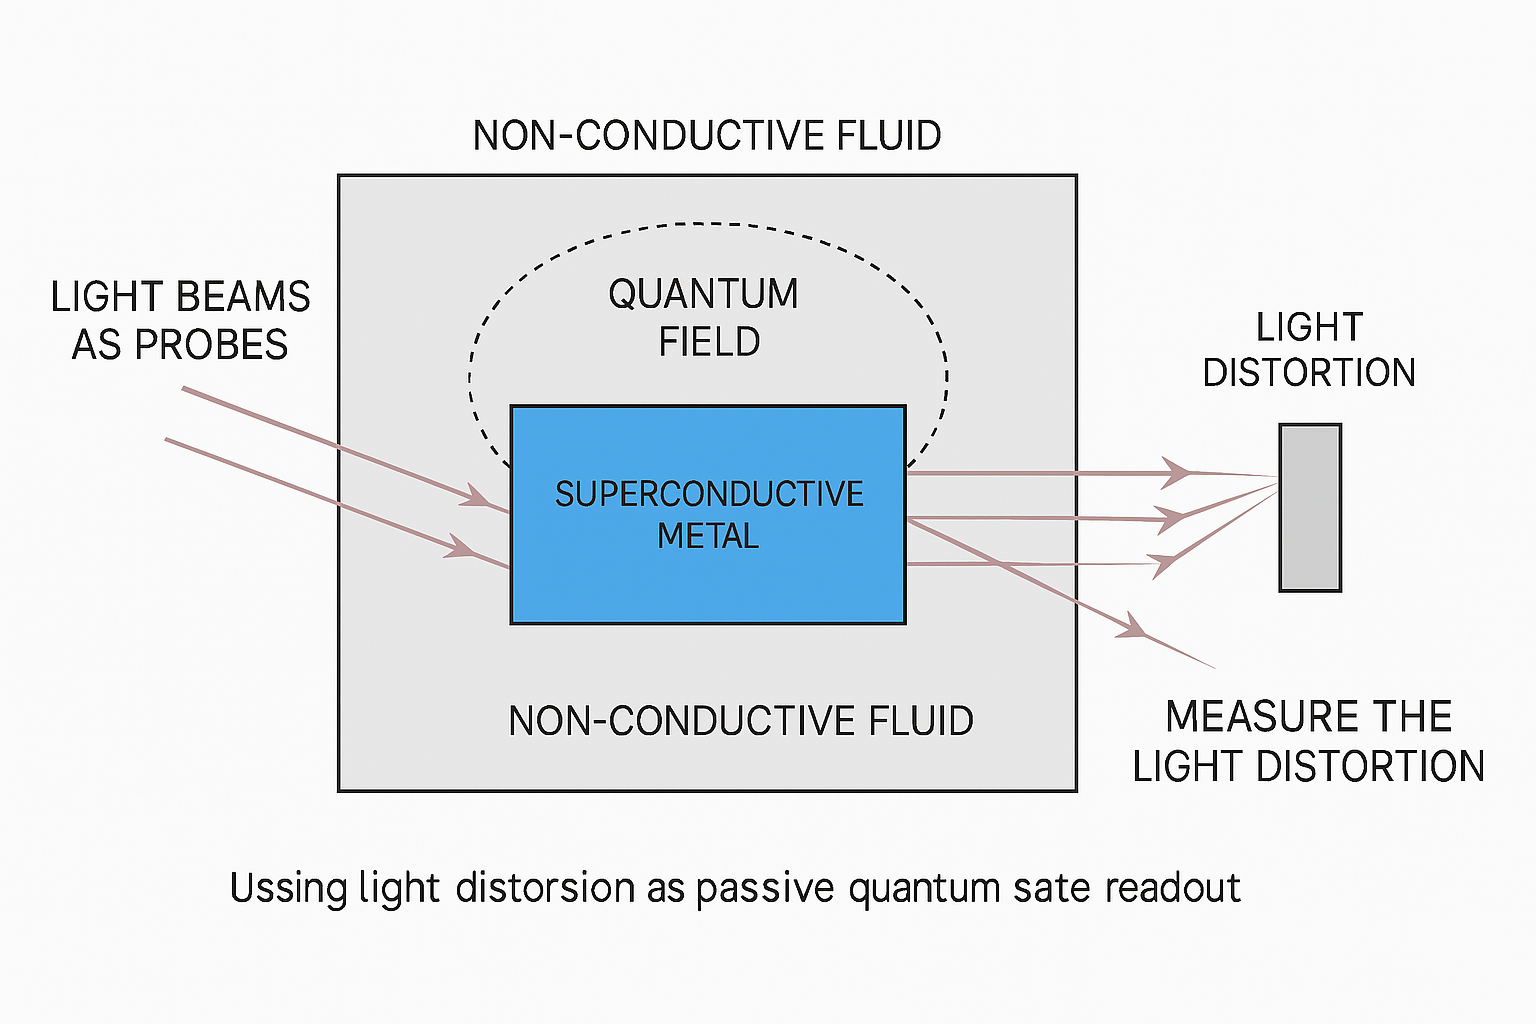
\includegraphics[width=0.85\textwidth]{images/qofas_schematic.png}
  \caption{QOFAS system schematic showing superconducting core, fluidic medium, and optical path.}
  \label{fig:qofas_schematic}
\end{figure}

\section{Core Principles of Detection}
Quantum field activity---even when unmeasured---modifies the local electromagnetic environment. In QOFAS, this influence manifests as:
\begin{itemize}
  \item Localized refractive index changes
  \item Birefringence via piezoelectric particle alignment
  \item Phase shift gradients in coherent light
  \item Subtle trajectory deformation of photons across the sensing shell
\end{itemize}
These phenomena are measurable using interferometers, Michelson setups, or laser cavity feedback loops.

\section{Application Domains}
\subsection{Qubit Detection}
QOFAS enables passive readout of superconducting, ion-trap, or photonic qubits. By tuning light paths across the qubit’s EM field region, the system can detect state transitions or tunneling events based on refractive deltas---without triggering wavefunction collapse.

\subsection{Quantum Networking}
In multi-node entangled systems, QOFAS shells surrounding individual qubit nodes may allow detection of entanglement-preserving field oscillations. When used at endpoints, these optical changes could provide indirect confirmation of link stability or drift.

\subsection{Entanglement-Based Encryption}
QOFAS proposes a way to confirm quantum key integrity by tracking the entangled state’s refractive signature. If an attacker collapses the state, the field distortion pattern would deviate sharply.

\subsection{Quantum Teleportation}
QOFAS may offer a verification layer at both transmission and reception ends, validating that the entangled state persists until the classical message arrives.

\subsection{Fusion Reactor Diagnostics}
QOFAS can operate as a passive diagnostic layer to detect phase displacement patterns in real-time, enabling visualization of magnetic boundary shifts or ELM precursors.

\begin{figure}[h!]
  \centering
  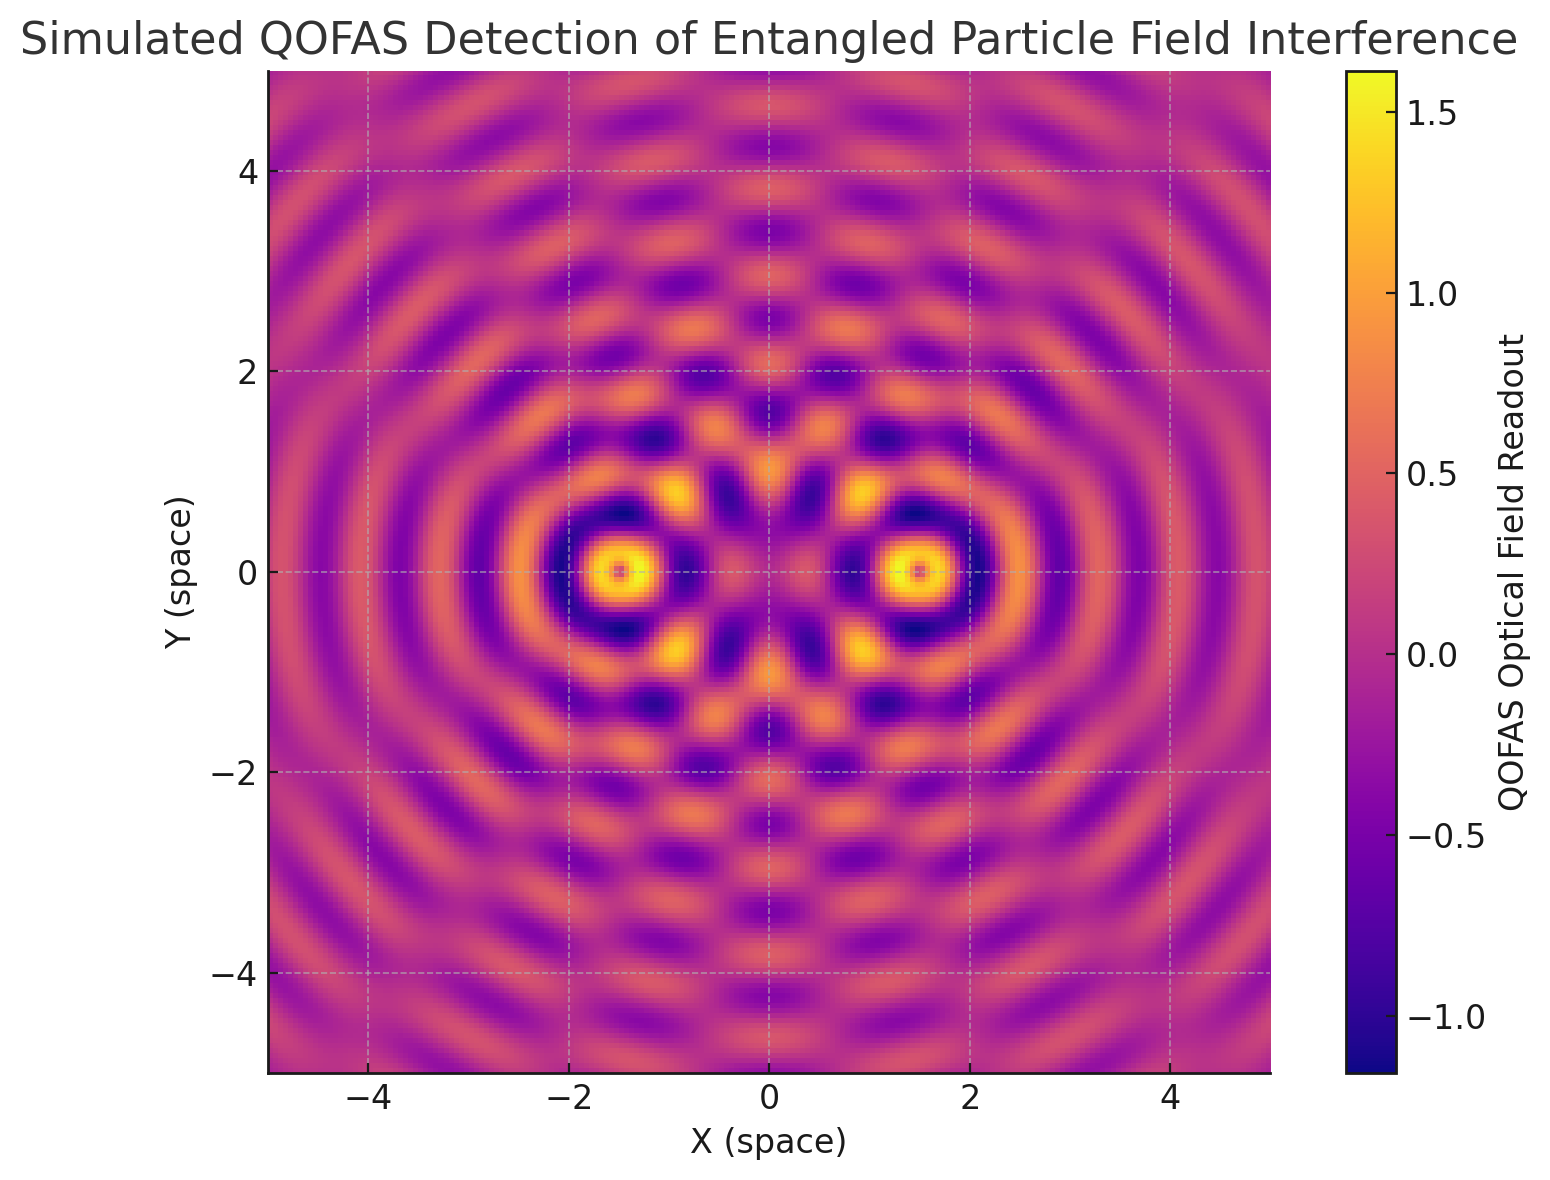
\includegraphics[width=0.85\textwidth]{images/entanglement_field_simulation.png}
  \caption{Simulation of entangled field interference pattern using Gaussian decay and cosine modulation.}
  \label{fig:entanglement_simulation}
\end{figure}

\section{Observables \\& Equations}
\textbf{Phase Shift:} \[ \Delta \phi = \frac{2 \pi n L}{\lambda} \]
\textbf{Index Perturbation:} \[ \Delta n = \alpha E^2 \]
\textbf{Fringe Displacement:} \[ \Delta x \propto \Delta \phi \cdot N_{passes} \]
\textbf{Resonant Frequency:} \[ f_{res} \propto \frac{1}{2 \pi} \sqrt{\frac{k_{eff}}{m}} \]

\begin{figure}[h!]
  \centering
  \includegraphics[width=0.85\textwidth]{images/qofas_concept_diagram.png}
  \caption{QOFAS Concept Diagram illustrating fluidic shell sensitivity, photon trajectory deformation, and potential applications.}
  \label{fig:qofas_concept}
\end{figure}

\section{Simulation Framework}
\begin{itemize}
  \item Entanglement Field Interference: Gaussian field decays modulated by cosine oscillation
  \item Particle-Field Response: Monte Carlo simulations of alignment and angular scattering
  \item Light Path Distortion: Beam propagation and FDTD modeling for phase delay
\end{itemize}

\section{Engineering and Deployment}
\begin{itemize}
  \item QOFAS shells can be integrated into cryogenic qubit environments
  \item Fusion diagnostics can operate within vacuum chamber optics
  \item Future models may incorporate photonic crystal fibers for in-line readout
\end{itemize}

\section{Conclusion}
QOFAS introduces a promising pathway toward non-destructive quantum state monitoring, enabling a layer of passive, refractive-based observation for highly sensitive systems. By capturing and amplifying naturally occurring optical field distortions, QOFAS has the potential to support a new generation of diagnostics in both quantum computing and high-energy physics domains.

\section*{References}
\begin{itemize}
  \item Braginsky, V. B., \& Khalili, F. Y. (1996). Quantum Non-demolition Measurements. Rev. Mod. Phys.
  \item Boyd, R. W. (2008). Nonlinear Optics. Academic Press.
  \item Wesson, J. (2011). Tokamaks. Oxford University Press.
  \item Lloyd, S. (2000). Ultimate physical limits to computation. Nature.
  \item Nielsen, M. A., \& Chuang, I. L. (2010). Quantum Computation and Quantum Information. Cambridge University Press.
\end{itemize}

\end{document}
